\chapter{Results and Discussion}

\section{Experimental Setup}

The official experiment uses the two datasets, four classifiers, four noise types, and frozen severity levels described in Chapter~3. The primary metric is Macro F1 and the secondary metric is Accuracy. Every result is evaluated on a clean test set that was never corrupted and never used for fitting.

Table~\ref{tab:runplans} summarises the three official stages and their measured runtimes. The MVP stage is a small Breast Cancer run used for validation and calibration. Stage 2 covers both datasets and all fifteen combinations with seeds 0--2. Full covers both datasets and all fifteen combinations with seeds 0--9.

\begin{table}[H]
\centering
\caption{Official run plans and measured runtimes.}
\label{tab:runplans}
\footnotesize
\begin{tabular}{p{1.1cm}p{1.9cm}p{2.4cm}p{1.1cm}p{1.4cm}p{1.9cm}}
\toprule
\textbf{Stage} & \textbf{Datasets} & \textbf{Combinations} & \textbf{Seeds} & \textbf{Fits} & \textbf{Runtime} \\
\midrule
MVP & Breast Cancer & 4 singles + label + gaussian & 0--2 & 312 & 22.2 s \\
Stage 2 & Both & All 15 & 0--2 & 1,824 & 215.3 s \\
Full & Both & All 15 & 0--9 & 6,080 & 703.8 s \\
\bottomrule
\end{tabular}
\end{table}

All 6,080 Full fits completed with status \texttt{ok} and zero error rows. The mean fit time was 0.1038 seconds and the maximum was 1.1598 seconds. The run used Python 3.11.9 on a Windows workstation without a GPU. The severity table was frozen before Stage 2 with configuration hash \texttt{bc9362\ldots}, methodology version 1.0.0, and levels version 1.0.0. A reproducibility subset of 112 fits was re-run and matched the original results exactly, and SHA-256 checksums were written for the final raw results and manifest.

The split sizes were 398 training and 171 test samples for Breast Cancer, and 1,257 training and 540 test samples for Digits. The same split was reused for every model and noise setting within a dataset and seed, which makes the comparisons paired.

\section{Results}

\subsection{Clean Baselines}

Table~\ref{tab:baselines} reports the clean level-0 baselines and the 90\% thresholds. The baselines are the reference against which every noisy result is compared.

\begin{table}[H]
\centering
\caption{Clean baselines and breaking thresholds (mean over ten seeds).}
\label{tab:baselines}
\small
\begin{tabular}{p{2.3cm}p{3.4cm}p{2.0cm}p{2.4cm}p{2.0cm}}
\toprule
\textbf{Dataset} & \textbf{Model} & \textbf{Baseline F1} & \textbf{Baseline Accuracy} & \textbf{Threshold F1} \\
\midrule
Breast Cancer & Logistic Regression & 0.9700 & 0.9719 & 0.8730 \\
Breast Cancer & SVM (RBF) & 0.9668 & 0.9690 & 0.8701 \\
Breast Cancer & Decision Tree & 0.9272 & 0.9316 & 0.8345 \\
Breast Cancer & Random Forest & 0.9547 & 0.9579 & 0.8592 \\
\midrule
Digits & Logistic Regression & 0.9697 & 0.9696 & 0.8727 \\
Digits & SVM (RBF) & 0.9813 & 0.9813 & 0.8831 \\
Digits & Decision Tree & 0.8420 & 0.8420 & 0.7578 \\
Digits & Random Forest & 0.9747 & 0.9748 & 0.8773 \\
\bottomrule
\end{tabular}
\end{table}

On Breast Cancer, Logistic Regression has the highest clean Macro F1 (0.9700), followed closely by SVM (0.9668) and Random Forest (0.9547). The Decision Tree is the weakest at 0.9272. On Digits, SVM is strongest (0.9813), followed by Random Forest (0.9747) and Logistic Regression (0.9697); the Decision Tree is again the weakest at 0.8420. The Decision Tree's lower baseline means that its threshold is also lower, so its early breaking points are not merely an artefact of a stricter absolute threshold.

\subsection{Breaking Points for Single Noise}

Table~\ref{tab:singlebp} reports the breaking level for each dataset, model, and single noise. ``NR'' means that the model did not reach the threshold by level 5.

\begin{table}[H]
\centering
\caption{Breaking levels for the four single-noise combinations (NR = not reached).}
\label{tab:singlebp}
\small
\begin{tabular}{llcccc}
\toprule
\textbf{Dataset} & \textbf{Model} & \textbf{Label} & \textbf{Gaussian} & \textbf{Outliers} & \textbf{Missing} \\
\midrule
Breast Cancer & Logistic Regression & 5 & NR & NR & NR \\
Breast Cancer & SVM (RBF) & 5 & NR & NR & NR \\
Breast Cancer & Decision Tree & 2 & 5 & NR & NR \\
Breast Cancer & Random Forest & 5 & 5 & NR & NR \\
\midrule
Digits & Logistic Regression & 4 & NR & NR & NR \\
Digits & SVM (RBF) & NR & NR & 5 & NR \\
Digits & Decision Tree & 2 & 3 & NR & 3 \\
Digits & Random Forest & NR & 5 & NR & NR \\
\bottomrule
\end{tabular}
\end{table}

The table reveals a clear ordering. Label noise is the most damaging single corruption. Averaged over the eight dataset--model pairs and treating ``not reached'' as level 6, the mean breaking level is 4.375 for label noise, 5.250 for Gaussian noise, 5.625 for missing values, and 5.875 for outliers. The corresponding mean absolute Macro F1 drop at level 5 is 0.1808 for label noise, 0.1251 for Gaussian noise, 0.0531 for missing values, and 0.0430 for outliers.

Label noise breaks every model on Breast Cancer and three of four models on Digits. Gaussian noise is the second most damaging corruption, and it breaks the Decision Tree and Random Forest on both datasets. Outliers and missing values rarely break a model in isolation, although missing values break the Decision Tree on Digits at level 3. SVM is unusually robust to label noise on Digits, where it does not reach the threshold by level 5, but it is the only model that breaks under outliers alone on Digits, at level 5.

\subsection{Compound-Noise Effects}

Compound noise is consistently more harmful than single noise. Table~\ref{tab:compoundbp} reports the mean breaking level by number of noise types, again treating ``not reached'' as level 6.

\begin{table}[H]
\centering
\caption{Mean breaking level by noise-set size (NR = 6).}
\label{tab:compoundbp}
\small
\begin{tabular}{lcccc}
\toprule
\textbf{Dataset} & \textbf{Singles} & \textbf{Pairs} & \textbf{Triples} & \textbf{Four-way} \\
\midrule
Breast Cancer & 5.438 & 5.208 & 4.875 & 4.750 \\
Digits & 5.125 & 4.250 & 3.562 & 2.750 \\
Combined & 5.281 & 4.729 & 4.219 & 3.750 \\
\bottomrule
\end{tabular}
\end{table}

The monotonic decrease is the central empirical result of the project. On Breast Cancer, the mean breaking level falls from 5.438 for single noise to 5.208 for pairs, 4.875 for triples, and 4.750 for the four-way combination. On Digits the decline is much steeper: 5.125, 4.250, 3.562, and 2.750. The four-way combination is therefore the most damaging setting in the entire experiment, and the gap between the single-noise and four-way means is 1.531 levels when the two datasets are combined.

Table~\ref{tab:keycombos} reports the mean breaking level for selected combinations on each dataset. It shows that combinations containing label noise dominate the early-failure region, and that the four-way combination is the earliest-breaking combination on Digits.

\begin{table}[H]
\centering
\caption{Mean breaking level for selected combinations (NR = 6).}
\label{tab:keycombos}
\footnotesize
\begin{tabular}{lccc}
\toprule
\textbf{Combination} & \textbf{Breast Cancer} & \textbf{Digits} & \textbf{Combined} \\
\midrule
Label & 4.250 & 4.500 & 4.375 \\
Gaussian & 5.500 & 5.000 & 5.250 \\
Missing & 6.000 & 5.250 & 5.625 \\
Outliers & 6.000 & 5.750 & 5.875 \\
Label + Gaussian & 4.750 & 4.250 & 4.500 \\
Label + Gaussian + Missing & 4.500 & 3.500 & 4.000 \\
Label + Gaussian + Outliers & 4.750 & 3.500 & 4.125 \\
Label + Outliers + Missing & 4.500 & 3.750 & 4.125 \\
Gaussian + Outliers + Missing & 5.750 & 3.500 & 4.625 \\
Label + Gaussian + Outliers + Missing & 4.750 & 2.750 & 3.750 \\
\bottomrule
\end{tabular}
\end{table}

Across all 120 dataset--model--combination cells, 83 breaking points were reached and 37 were not. Of the reached breaking points, 8 occurred at level 2, 15 at level 3, 22 at level 4, and 38 at level 5. The distribution differs sharply between datasets. On Breast Cancer, 28 of the 36 reached breaking points occurred at level 5, which indicates a late and gradual failure. On Digits, only 10 of the 47 reached breaking points occurred at level 5, while 19 occurred at level 4, 12 at level 3, and 6 at level 2, which indicates earlier and more abrupt failure.

\subsection{Robustness Ranking}

Table~\ref{tab:robustness} reports the BPI, RS, and rank for the all-combinations and single-noise scopes. Higher BPI means that a model survives to a higher severity; higher RS means that it retains more of its baseline performance across levels.

\begin{table}[H]
\centering
\caption{Robustness ranking by BPI and RS.}
\label{tab:robustness}
\resizebox{\textwidth}{!}{%
\begin{tabular}{llcccccc}
\toprule
\textbf{Dataset} & \textbf{Model} & \textbf{BPI (all)} & \textbf{RS (all)} & \textbf{Rank} & \textbf{BPI (singles)} & \textbf{RS (singles)} & \textbf{Rank} \\
\midrule
Breast Cancer & Logistic Regression & 5.467 & 0.960 & 1 & 5.750 & 0.972 & 2 \\
Breast Cancer & SVM (RBF) & 5.467 & 0.958 & 2 & 5.750 & 0.976 & 1 \\
Breast Cancer & Random Forest & 5.400 & 0.957 & 3 & 5.500 & 0.968 & 3 \\
Breast Cancer & Decision Tree & 4.267 & 0.895 & 4 & 4.750 & 0.931 & 4 \\
\midrule
Digits & Random Forest & 4.800 & 0.922 & 1 & 5.750 & 0.975 & 1 \\
Digits & Logistic Regression & 4.667 & 0.925 & 2 & 5.500 & 0.953 & 3 \\
Digits & SVM (RBF) & 4.533 & 0.922 & 3 & 5.750 & 0.966 & 2 \\
Digits & Decision Tree & 2.800 & 0.747 & 4 & 3.500 & 0.862 & 4 \\
\bottomrule
\end{tabular}}
\end{table}

No single model dominates on both datasets. On Breast Cancer, Logistic Regression and SVM have the same all-combination BPI (5.467), and Logistic Regression is ranked first by the RS tie-break. On Digits, Random Forest is ranked first with BPI 4.800 and RS 0.922. The Decision Tree is last on both datasets, with a BPI of 4.267 on Breast Cancer and 2.800 on Digits. Its RS is also the lowest: 0.895 on Breast Cancer and 0.747 on Digits.

Averaged across the two datasets, Random Forest has the highest mean BPI (5.100), followed by Logistic Regression (5.067), SVM (5.000), and Decision Tree (3.533). Logistic Regression has the highest mean RS (0.9423), followed by Random Forest (0.9397), SVM (0.9396), and Decision Tree (0.8207). The two aggregate measures therefore agree on the weakest model and disagree slightly on the strongest, which is why both are reported.

\subsection{Synergy Analysis}

The synergy analysis compares the compound drop with the sum of the corresponding single-noise drops. A positive value means that the compound is worse than additive; a negative value means that it is less than additive. The analysis covers 440 compound cells: 11 compound combinations, 4 models, 2 datasets, and 5 levels.

Of the 440 cells, 124 (28.2\%) have positive synergy and 316 (71.8\%) have negative synergy. The mean synergy is negative on both datasets: $-0.0308$ on Breast Cancer and $-0.0105$ on Digits. At level 5, the mean is $-0.0711$ on Breast Cancer and $-0.0024$ on Digits. The general pattern is therefore sub-additive: the damage caused by compound noise is usually smaller than the sum of the damage caused by the same noises individually.

The exceptions are important. The largest positive synergy is 0.2958, for Random Forest on Digits with the four-way combination at level 5. The next largest are 0.1601 for SVM on Digits with label + Gaussian + outliers at level 5, and 0.0672 for SVM on Breast Cancer with label + Gaussian + outliers at level 5. These are cases in which the interaction between corruption types produces more damage than an additive model would predict. The floor-effect flag is set in two cases, both for the Decision Tree on Digits at level 5, where the sum of single-noise drops exceeds the baseline.

The practical implication is that compound noise is more damaging in absolute terms, but not necessarily more than additive. A simple additive projection can overestimate the total drop in most cells, while underestimating it in a small number of high-severity multiclass cells. Both the absolute effect and the interaction effect should therefore be reported.

\subsection{Figures}

Figures~\ref{fig:bc-f1} and~\ref{fig:digits-f1} show Macro F1 versus severity for each single noise. Each panel contains the four models, the mean over ten seeds, a shaded one-standard-deviation band, the 90\% threshold, and a red cross at the breaking point.

\begin{figure}[H]
\centering
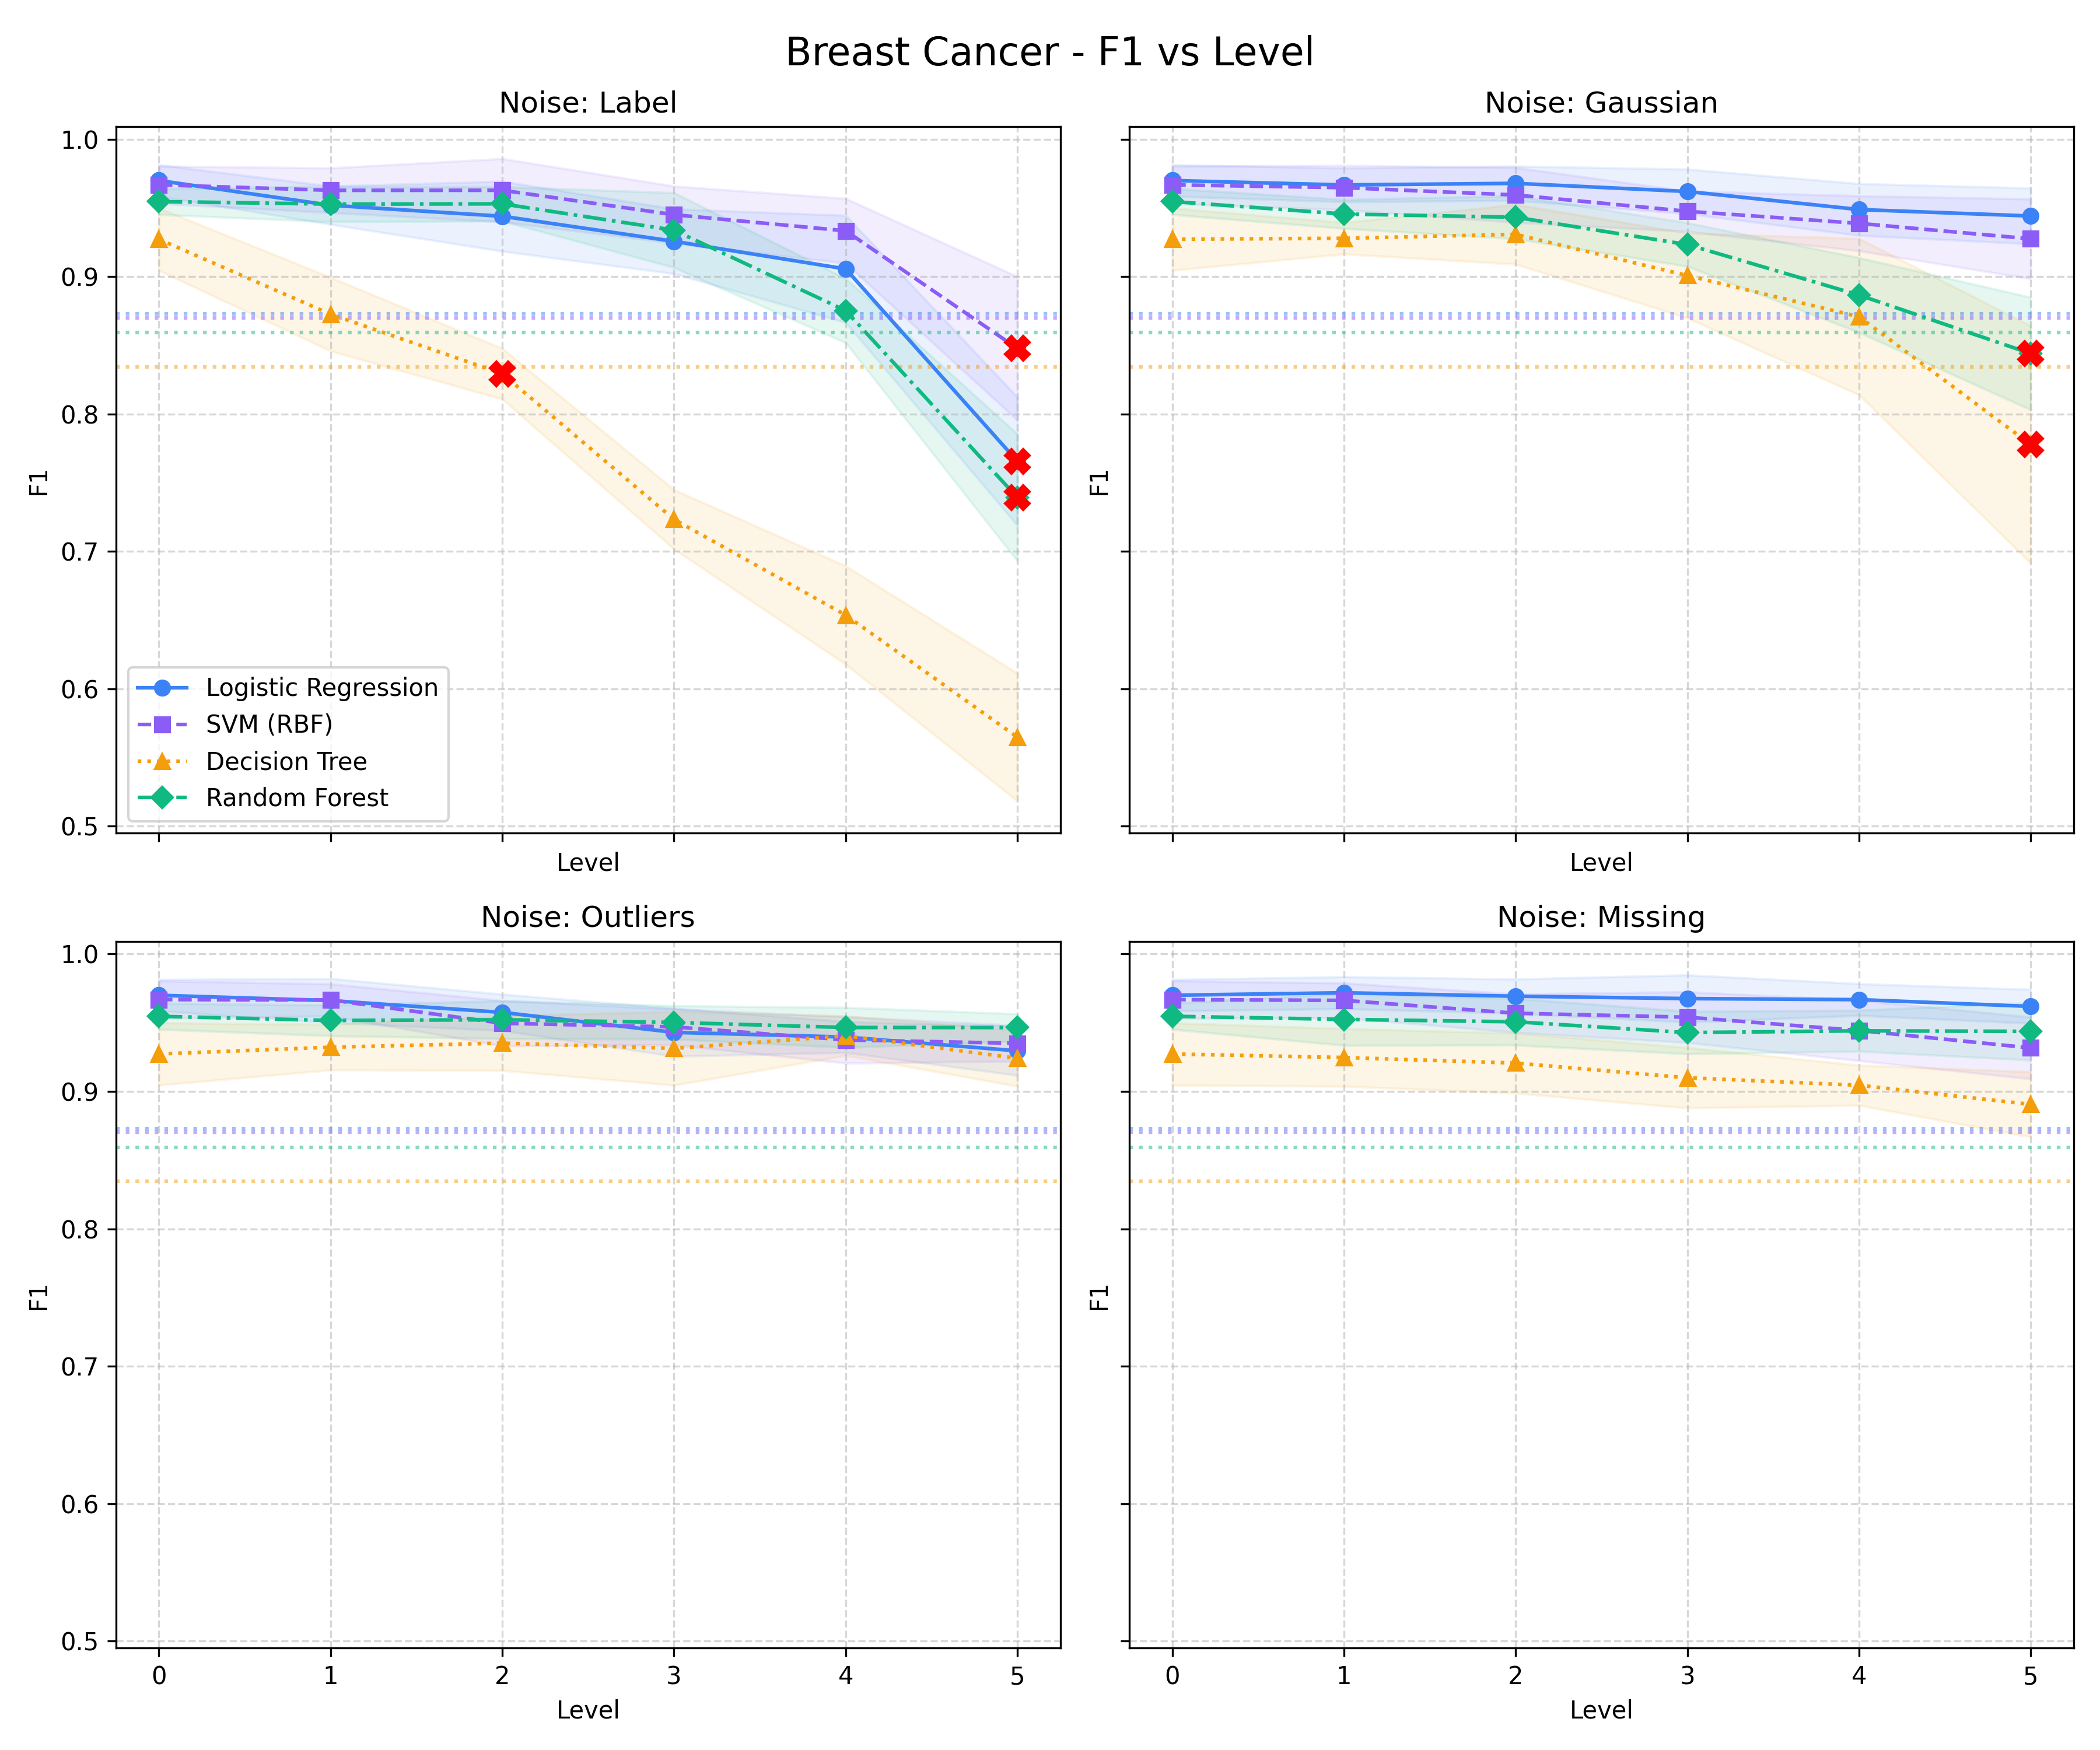
\includegraphics[width=0.95\textwidth]{figures/project_figures/bc-f1-vs-level.png}
\caption{Breast Cancer: Macro F1 versus severity level for the four single-noise combinations. The dotted lines are the 90\% thresholds and the red crosses mark breaking points.}
\label{fig:bc-f1}
\end{figure}

\begin{figure}[H]
\centering
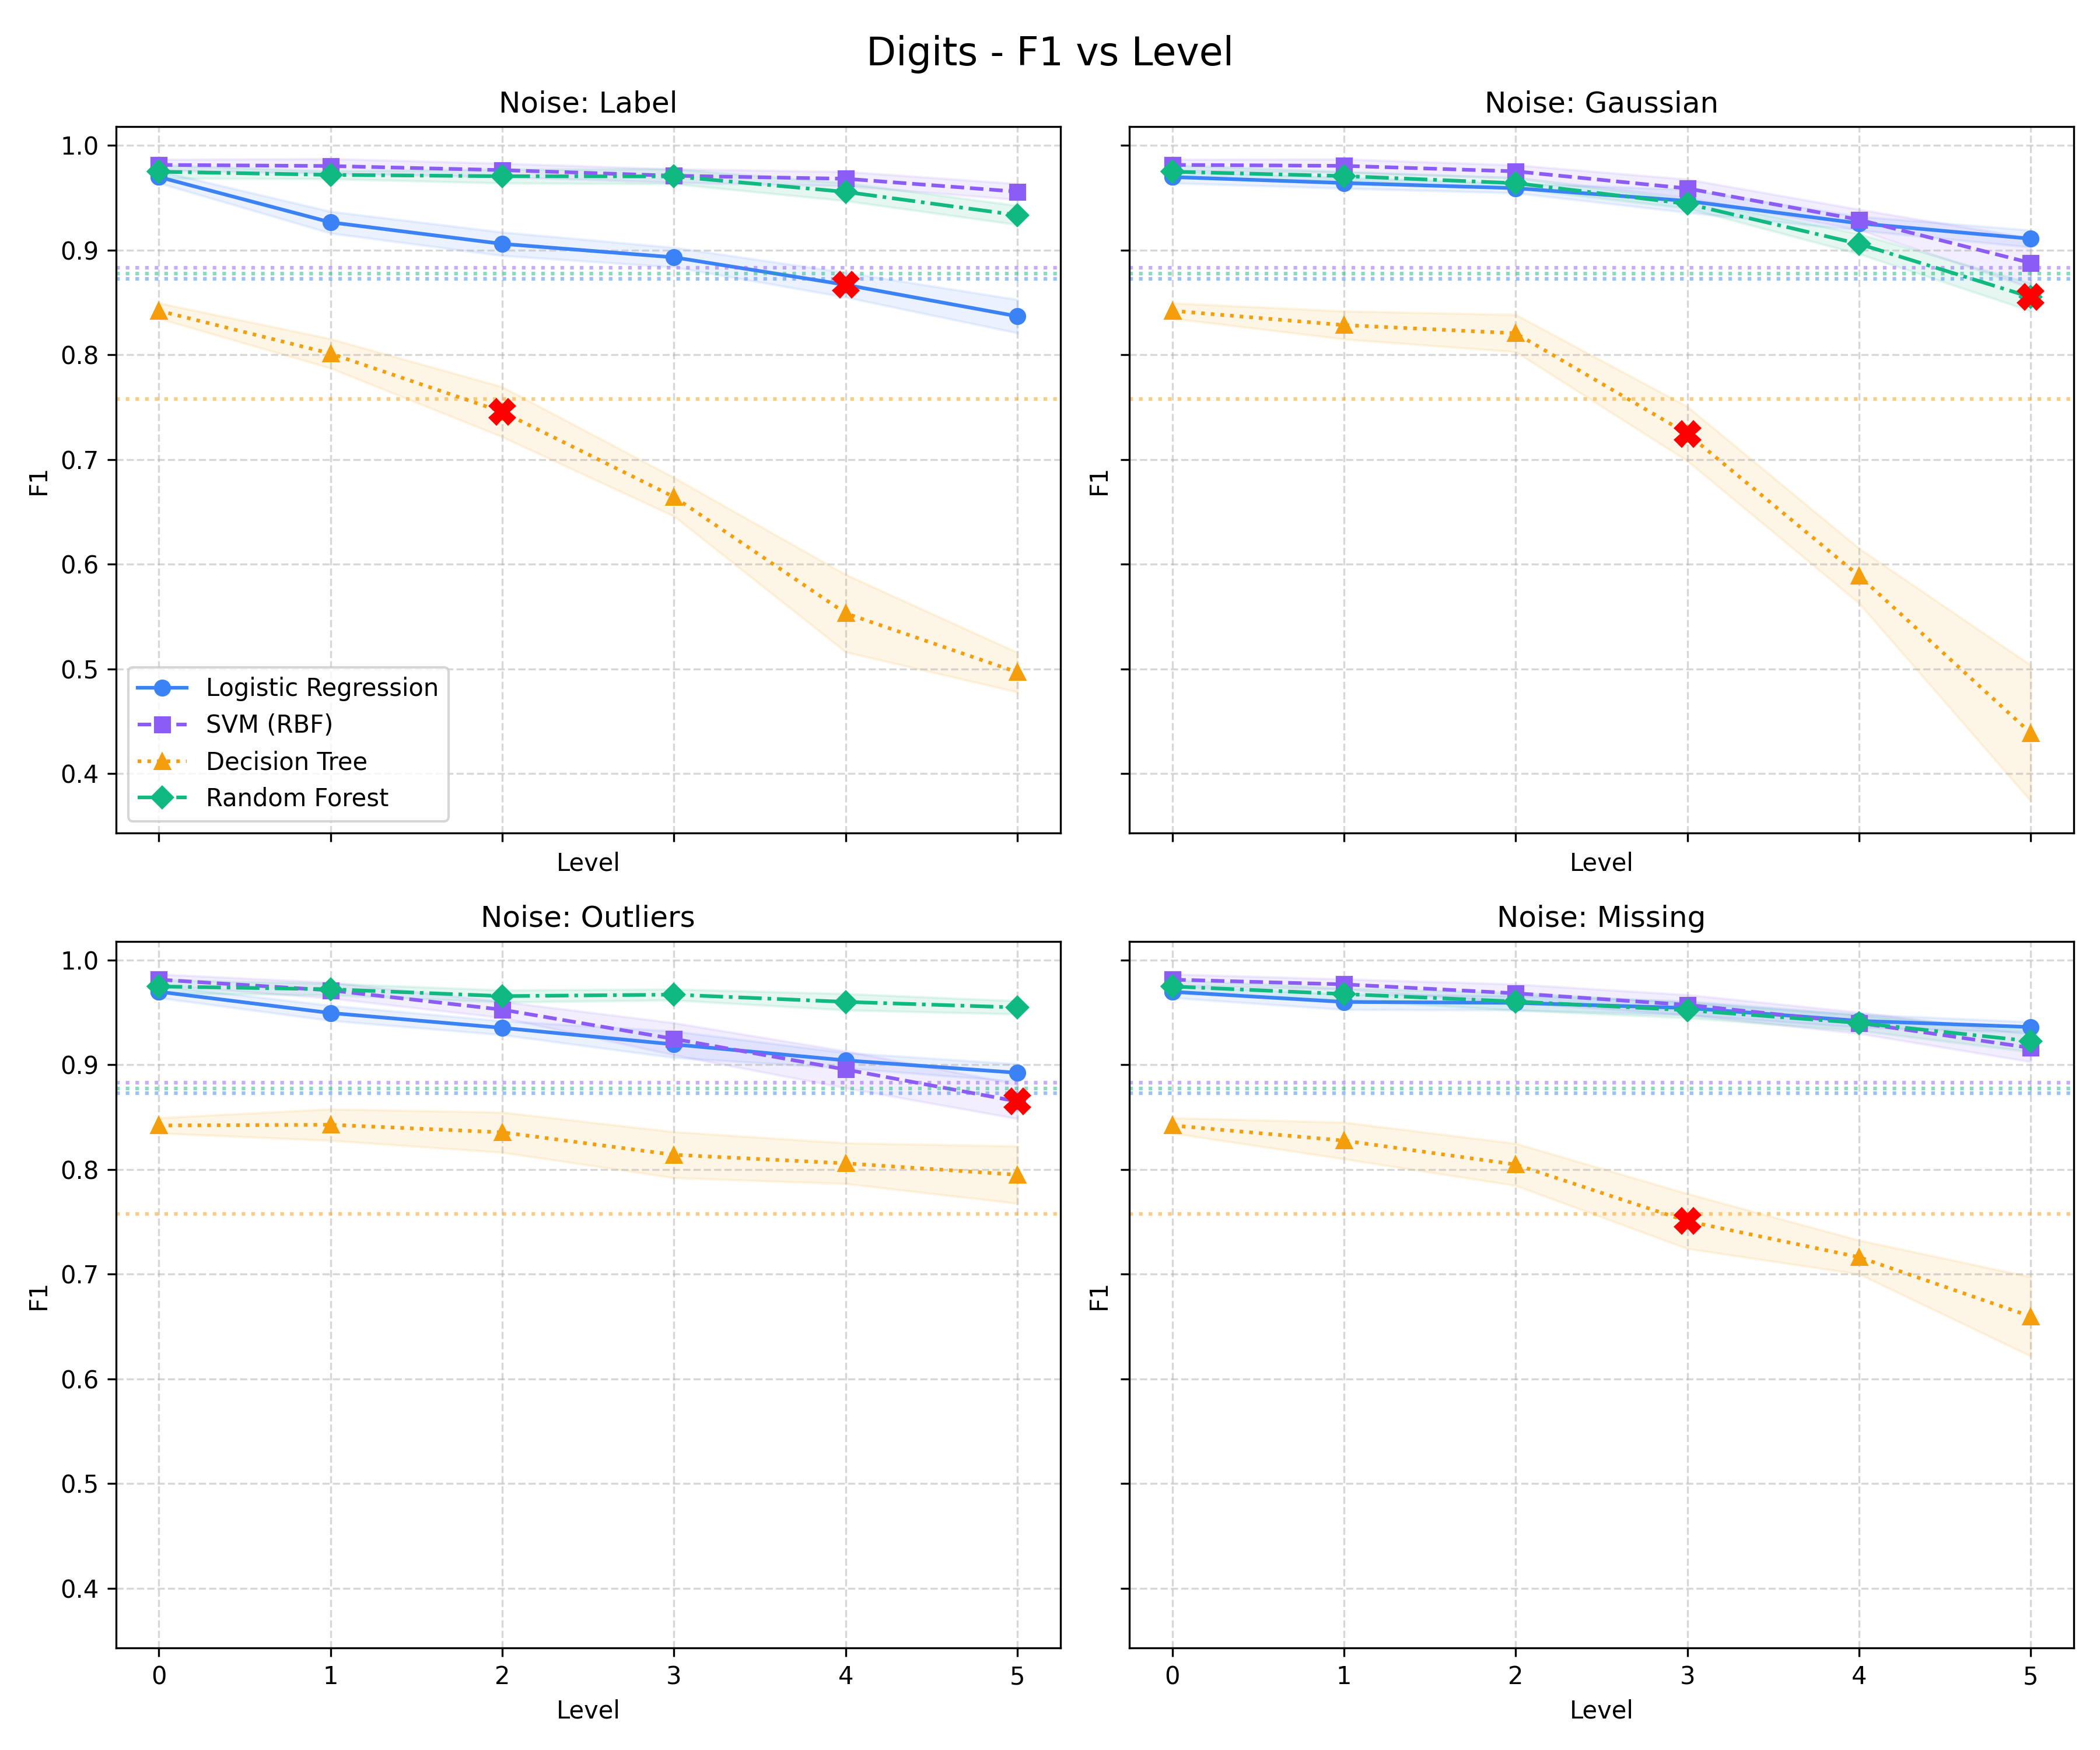
\includegraphics[width=0.95\textwidth]{figures/project_figures/digits-f1-vs-level.png}
\caption{Digits: Macro F1 versus severity level for the four single-noise combinations. The dotted lines are the 90\% thresholds and the red crosses mark breaking points.}
\label{fig:digits-f1}
\end{figure}

Figures~\ref{fig:bc-heat} and~\ref{fig:digits-heat} show the breaking level for all fifteen combinations and four models. Lighter cells indicate earlier failure, darker cells indicate later failure, and the value 6 means that the threshold was not reached.

\begin{figure}[H]
\centering
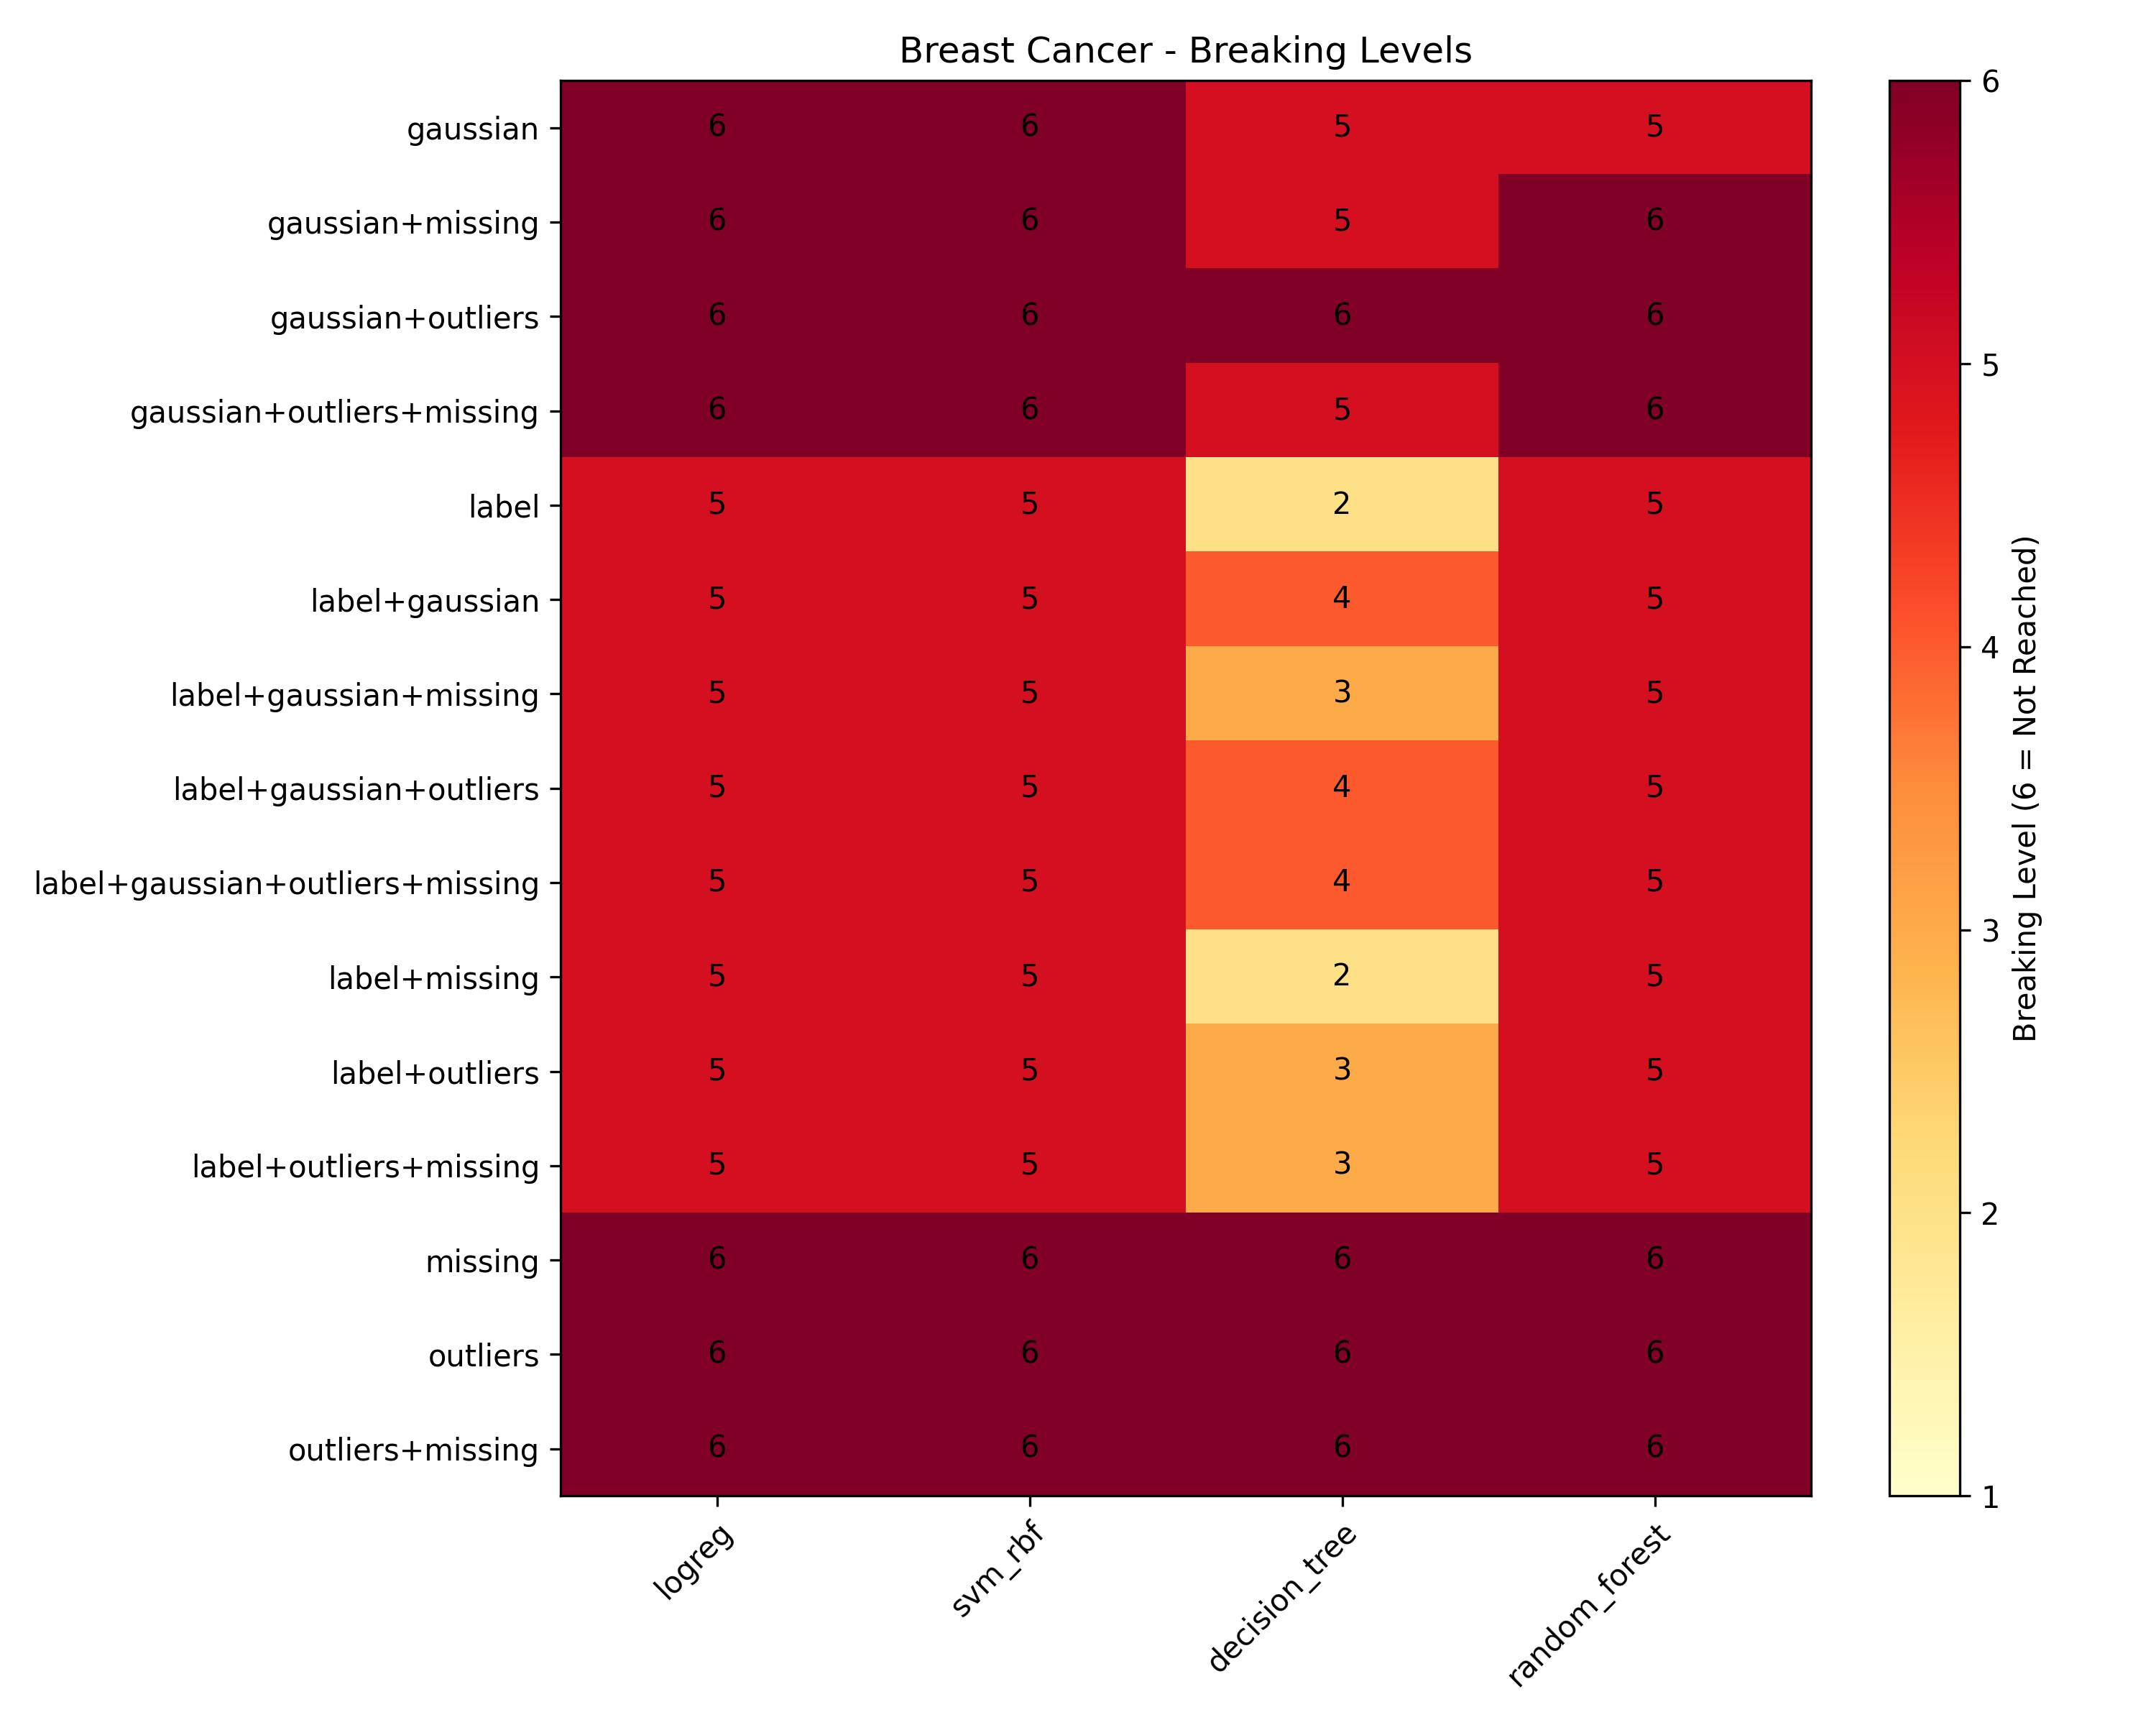
\includegraphics[width=0.82\textwidth]{figures/project_figures/bc-heatmap.png}
\caption{Breast Cancer: breaking level for every combination and model. Lighter cells fail earlier; 6 means not reached.}
\label{fig:bc-heat}
\end{figure}

\begin{figure}[H]
\centering
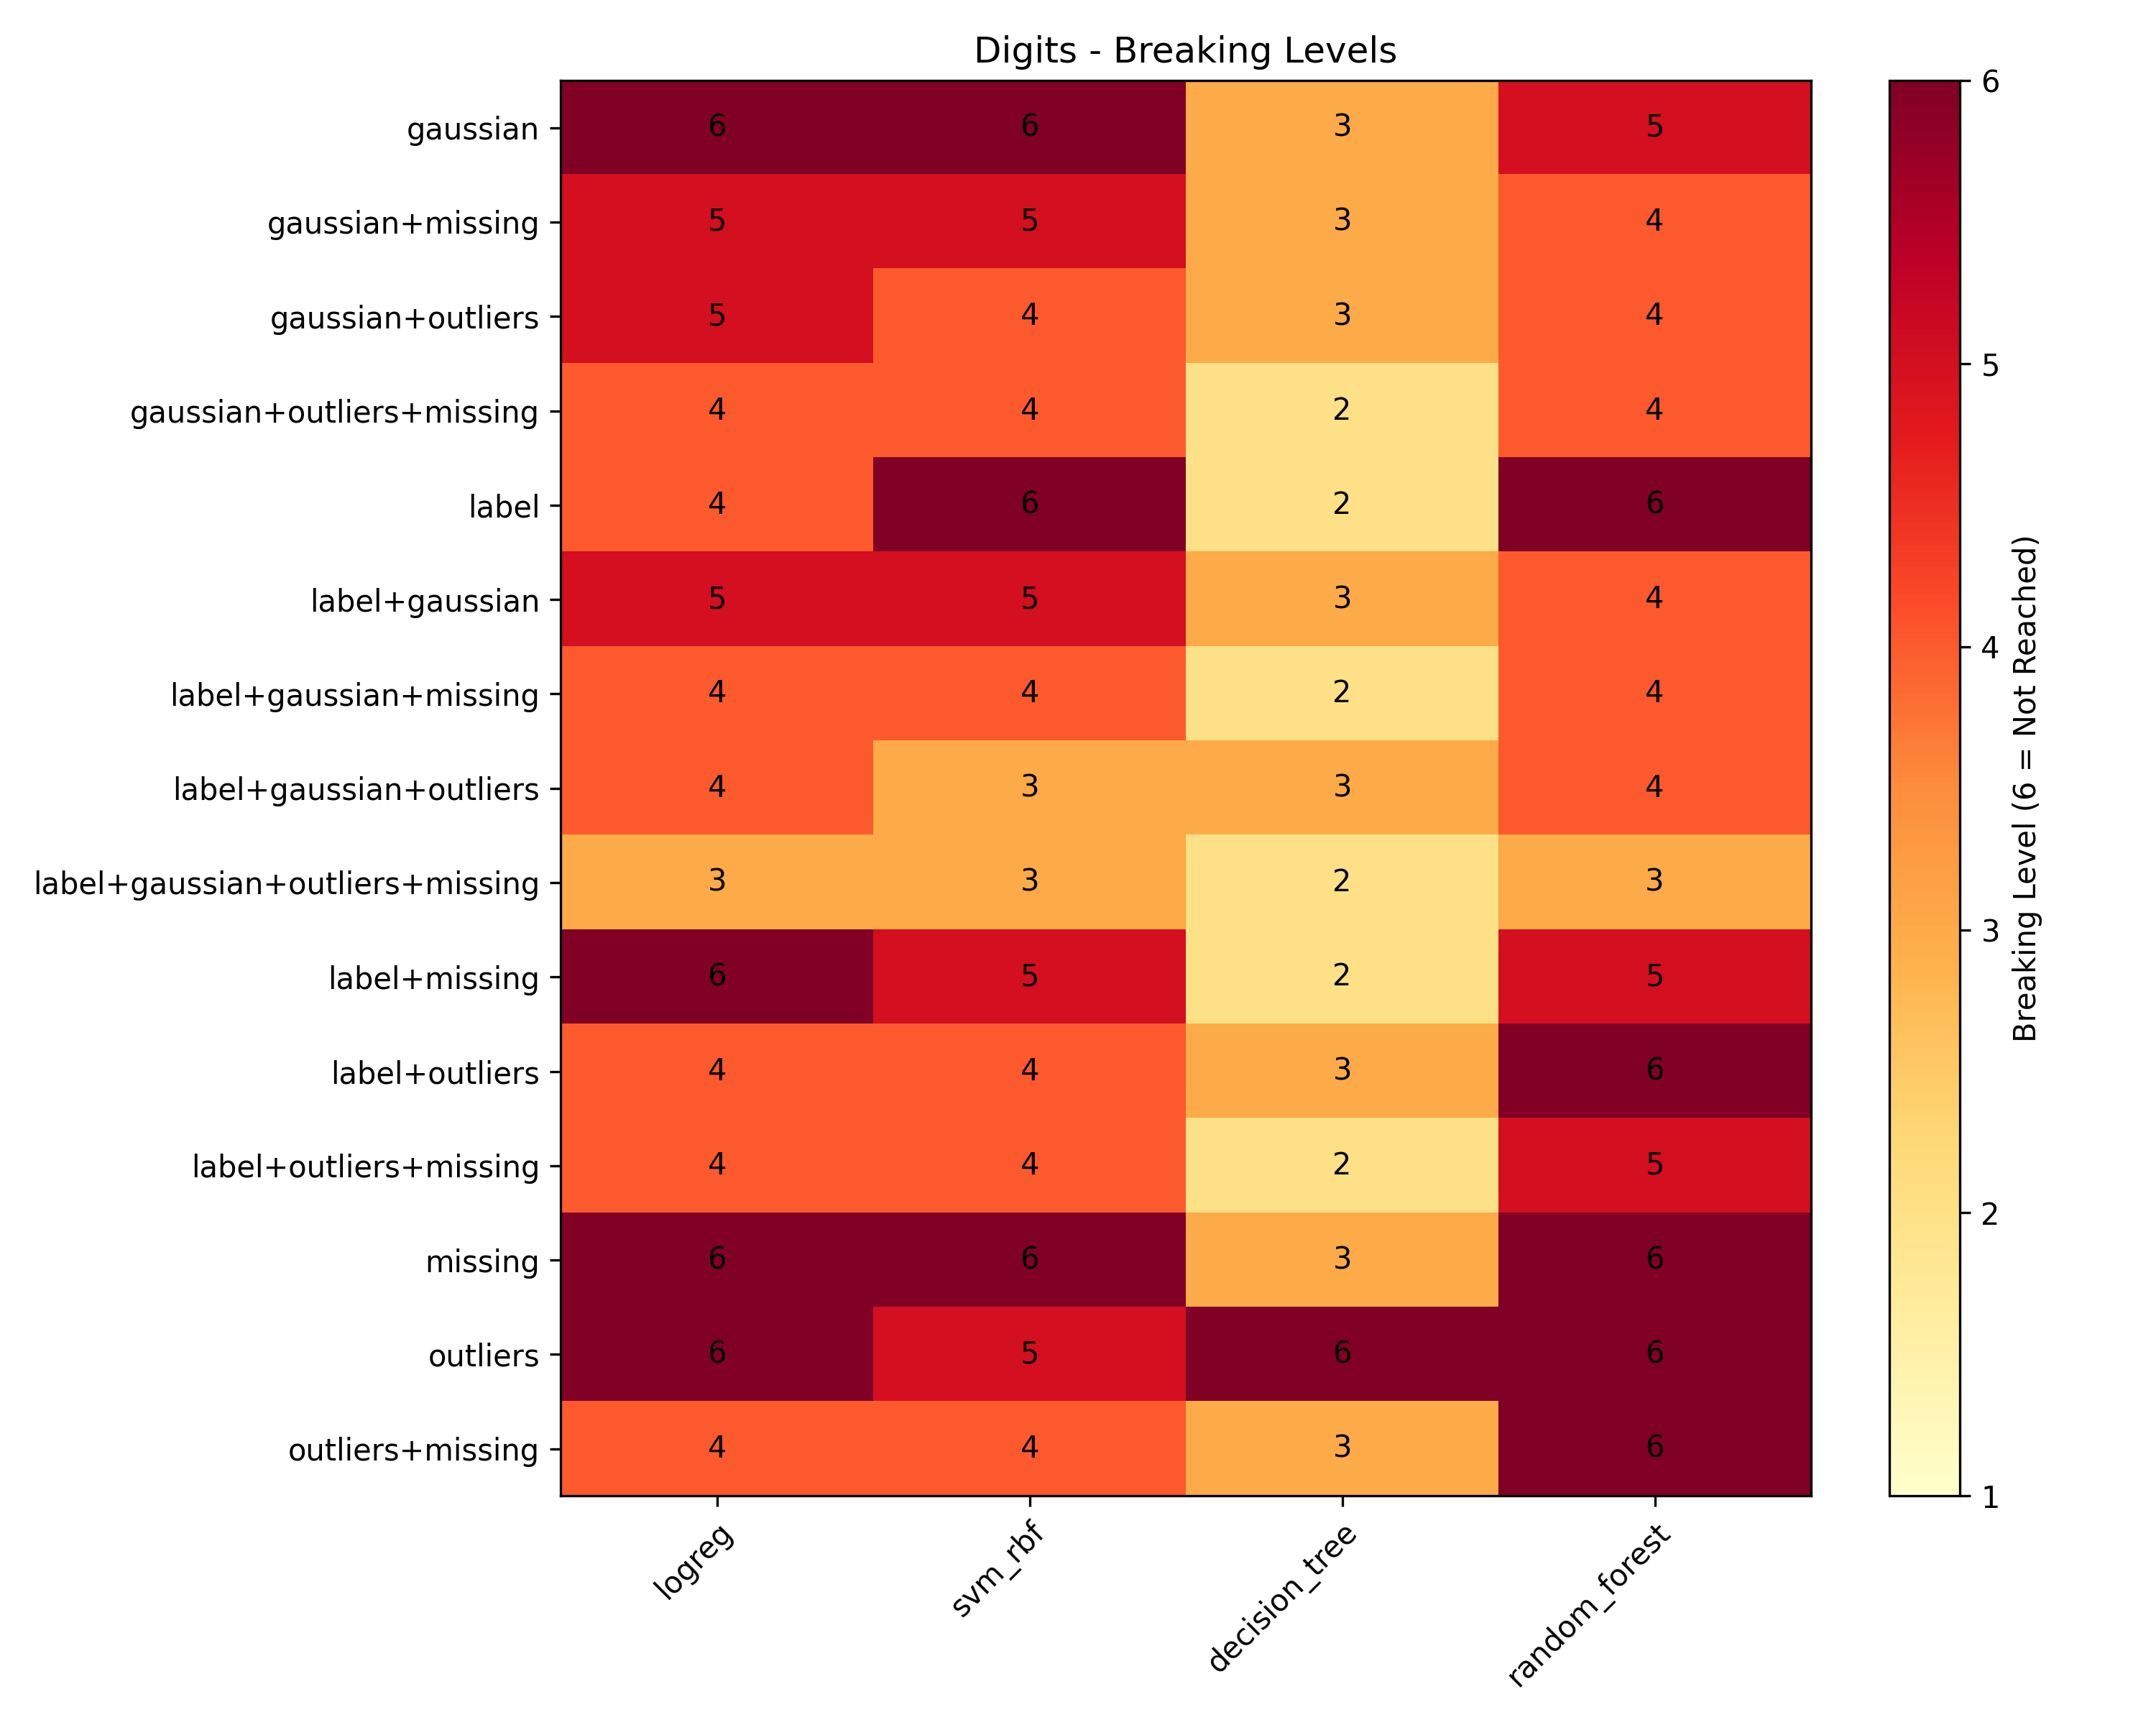
\includegraphics[width=0.82\textwidth]{figures/project_figures/digits-heatmap.png}
\caption{Digits: breaking level for every combination and model. The much lighter cells show earlier failure than on Breast Cancer.}
\label{fig:digits-heat}
\end{figure}

Figures~\ref{fig:bc-syn} and~\ref{fig:digits-syn} show the level-5 synergy for every compound combination and model. Positive bars indicate super-additive damage.

\begin{figure}[H]
\centering
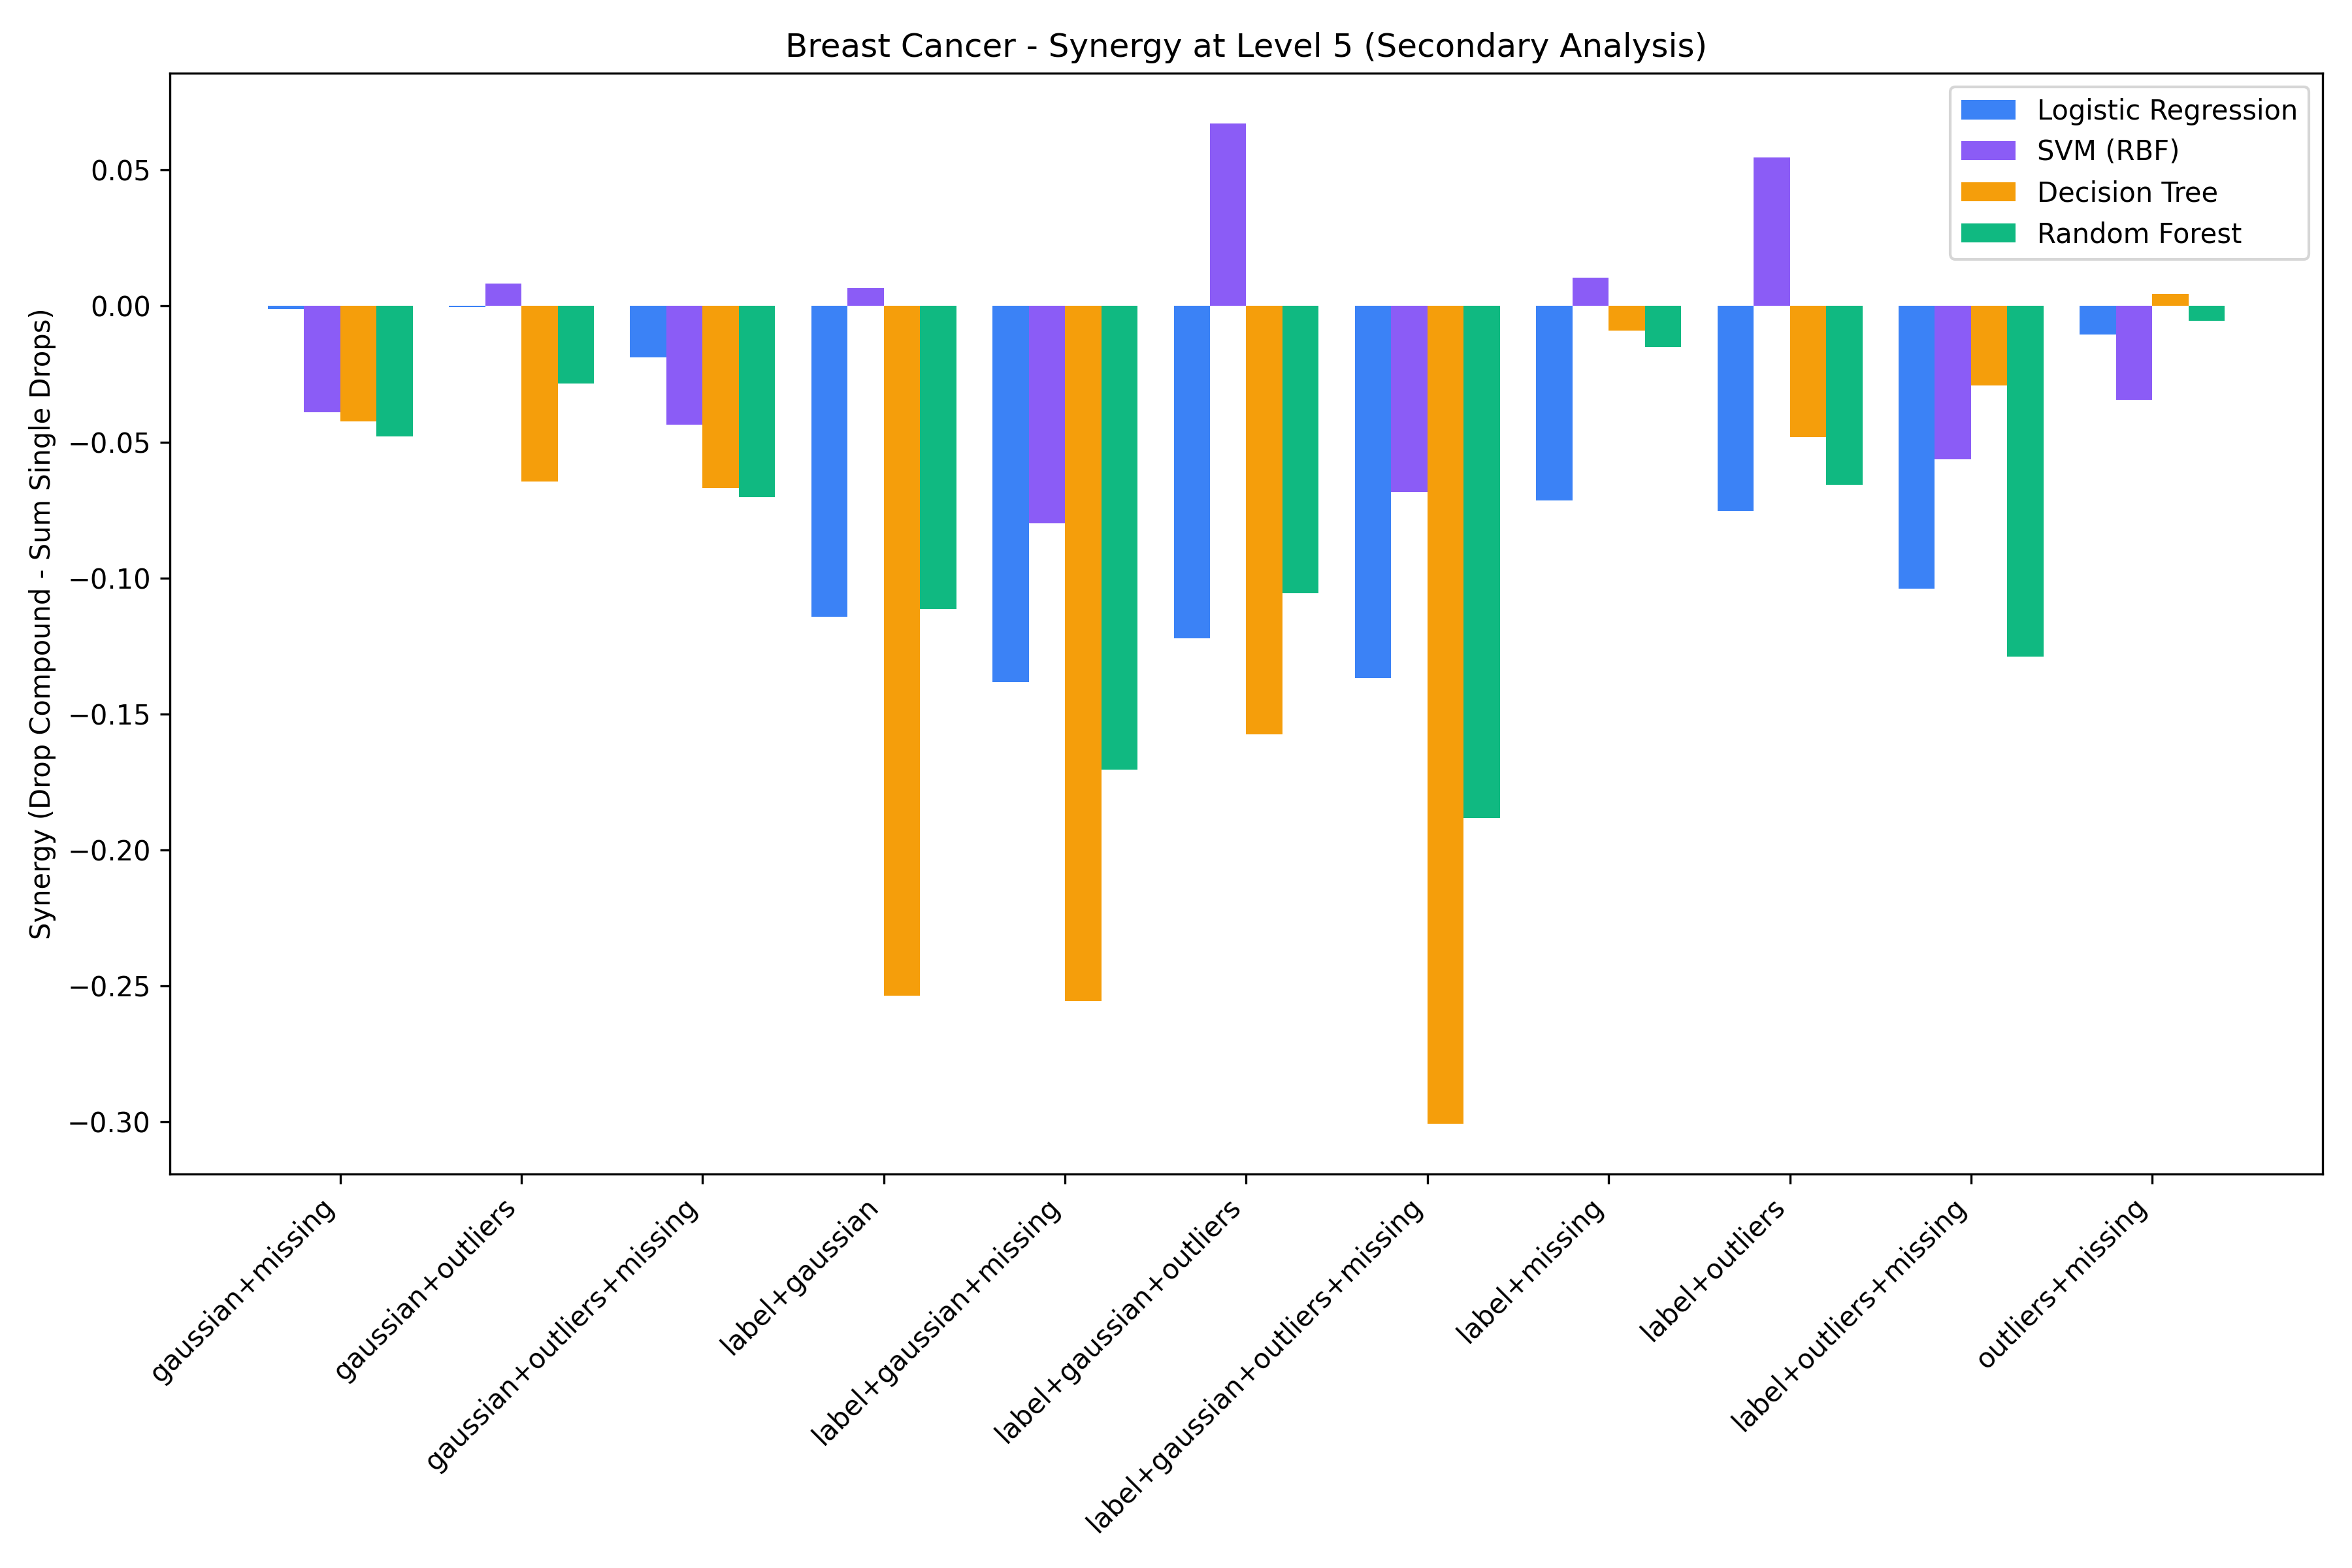
\includegraphics[width=0.95\textwidth]{figures/project_figures/bc-synergy.png}
\caption{Breast Cancer: synergy at level 5. Positive values mean that the compound drop exceeds the sum of single-noise drops.}
\label{fig:bc-syn}
\end{figure}

\begin{figure}[H]
\centering
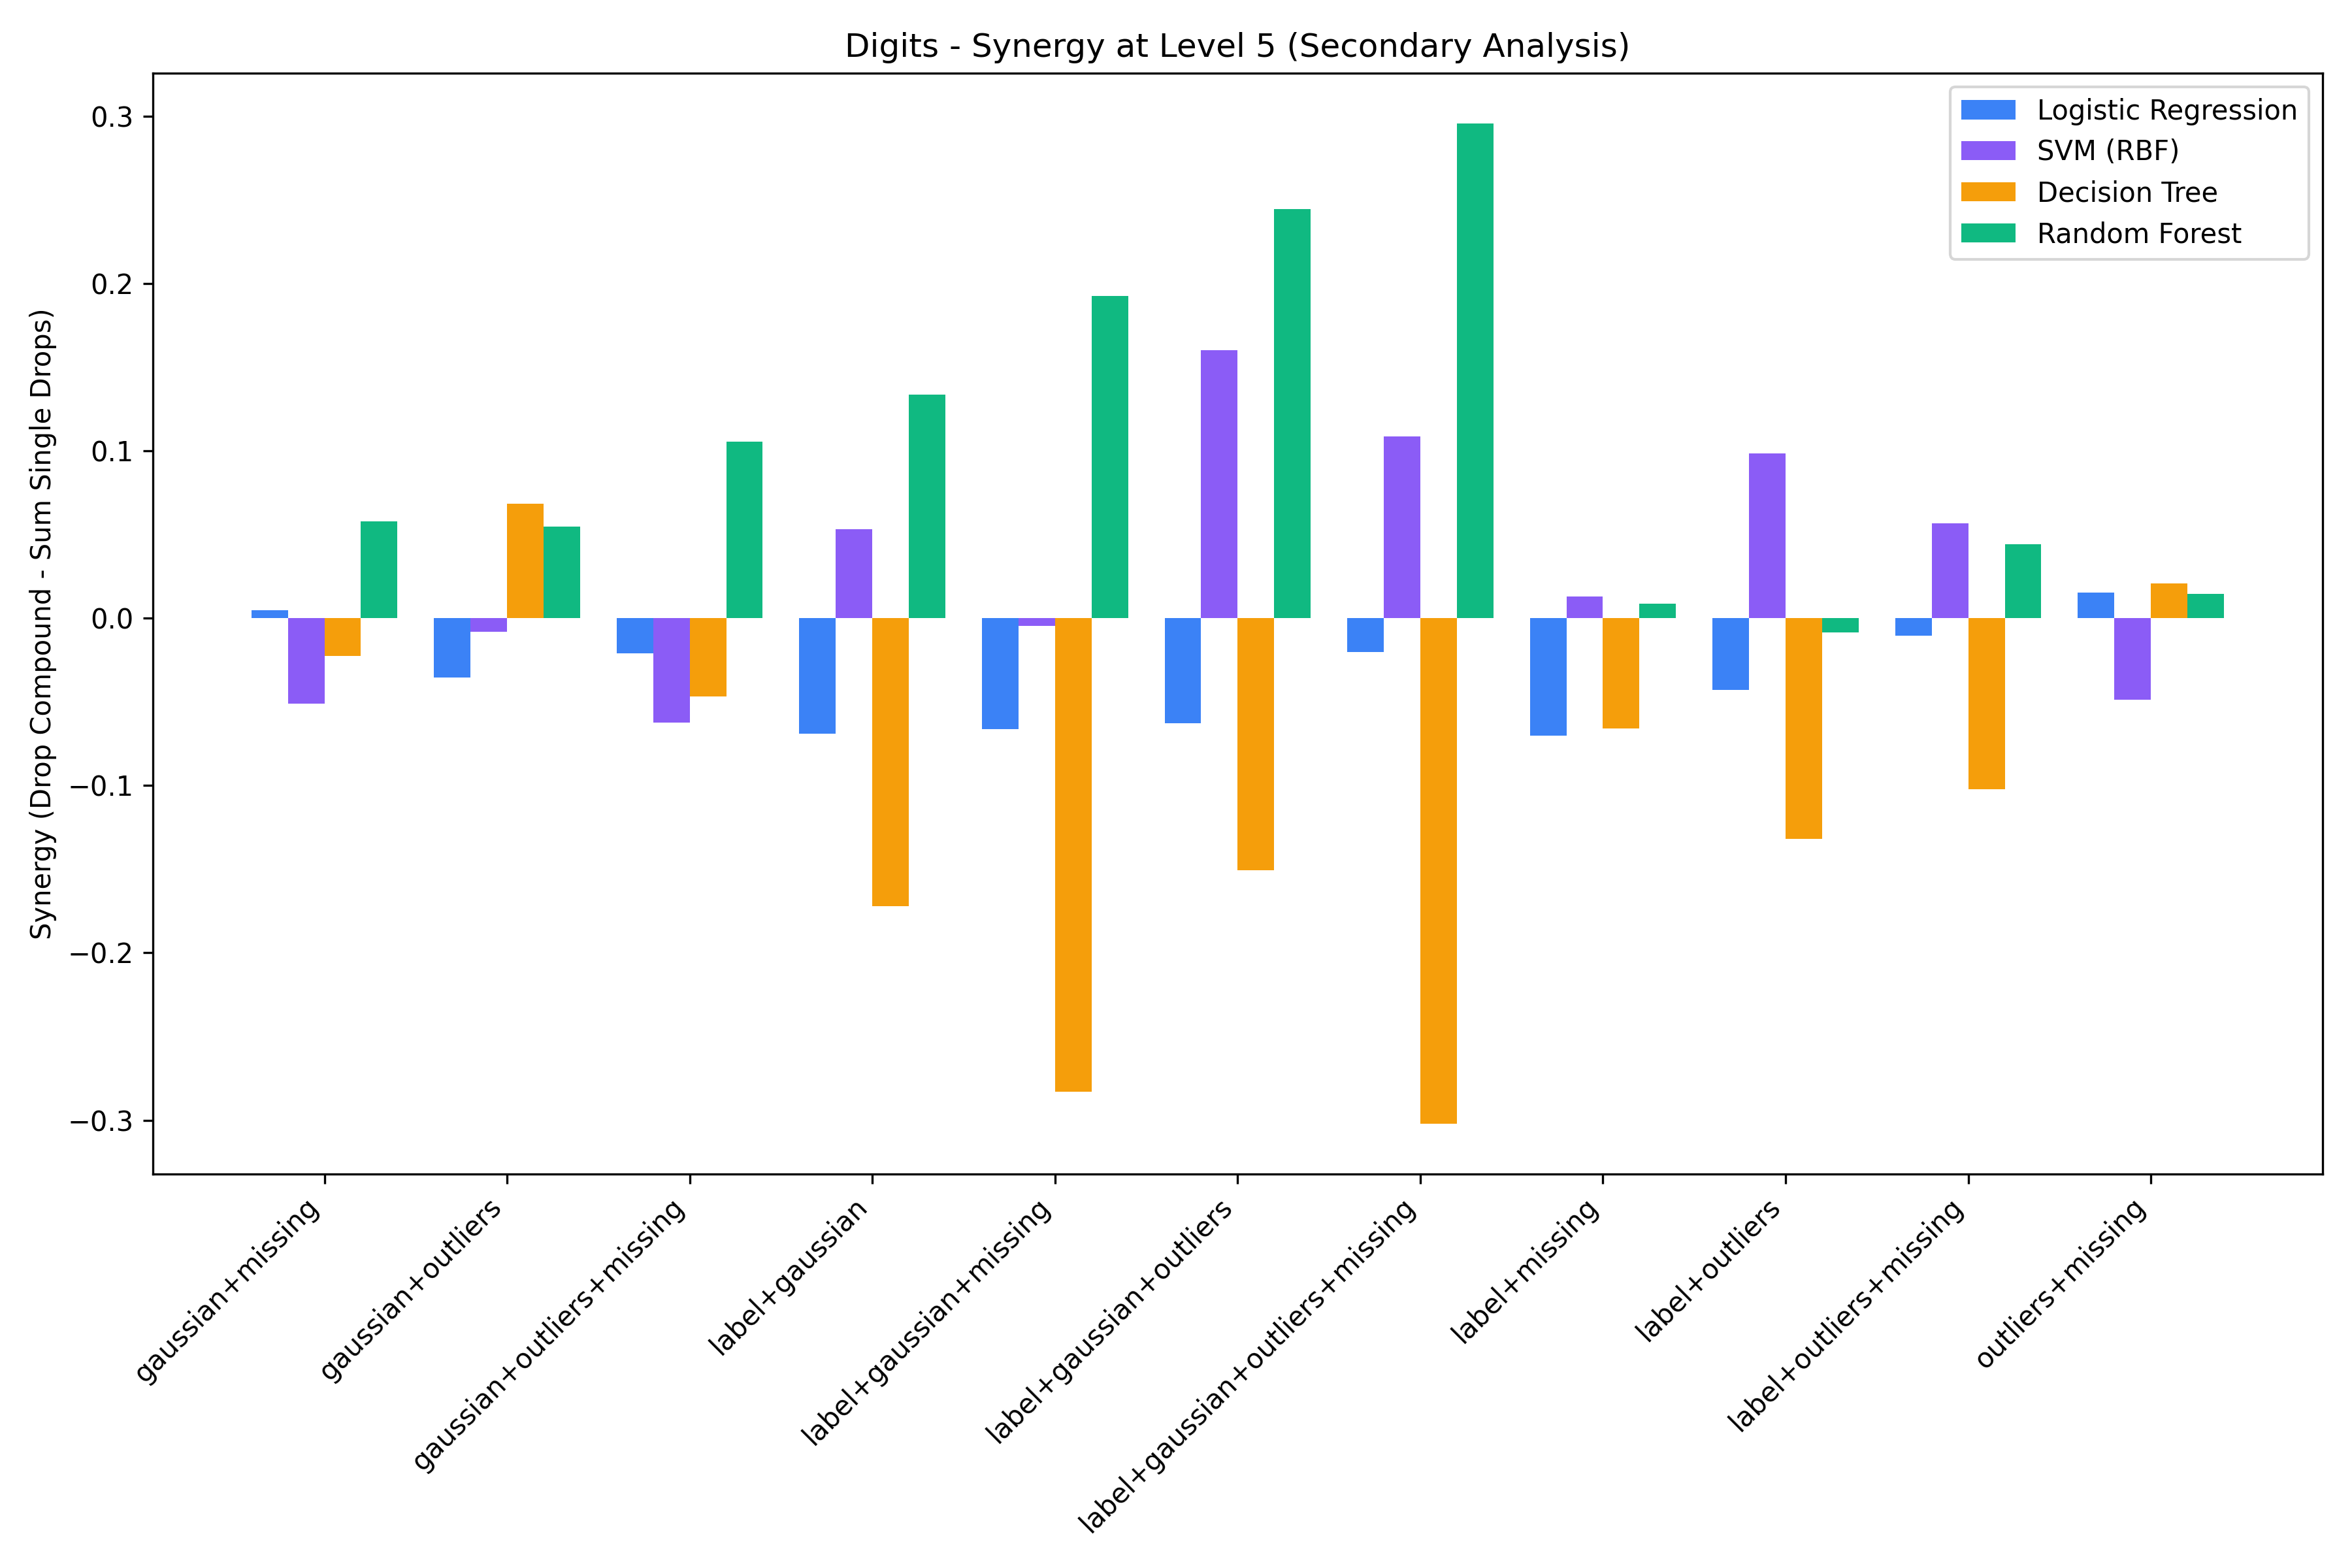
\includegraphics[width=0.95\textwidth]{figures/project_figures/digits-synergy.png}
\caption{Digits: synergy at level 5. The largest positive bars occur for high-severity combinations involving label and Gaussian noise.}
\label{fig:digits-syn}
\end{figure}

\section{Performance Analysis}

\subsection{Answers to the Research Questions}

\textbf{Q1: Which model is most robust overall?} There is no single winner on every measure. Random Forest has the highest mean BPI across the two datasets (5.100), while Logistic Regression has the highest mean RS (0.9423). On Breast Cancer, Logistic Regression is ranked first in the all-combination scope, and SVM is ranked first in the single-noise scope. On Digits, Random Forest is ranked first in both scopes. The Decision Tree is unambiguously the least robust model: it is last on both datasets, its BPI is 3.533 on average, and its RS is 0.8207. The practical answer therefore depends on the objective. If survival to a higher severity is the priority, Random Forest is the best overall choice. If retained performance across levels is the priority, Logistic Regression is marginally better. Both are preferable to the Decision Tree.

\textbf{Q2: Which noise type hurts most?} Label noise is the most damaging single corruption. Its mean breaking level is 4.375, compared with 5.250 for Gaussian noise, 5.625 for missing values, and 5.875 for outliers. Its mean level-5 Macro F1 drop is 0.1808, compared with 0.1251, 0.0531, and 0.0430 respectively. Label noise is also the only single corruption that breaks every model on Breast Cancer. Gaussian noise is the second most damaging corruption. Outliers and missing values are comparatively benign in isolation, but they can become harmful when combined with label noise or when they interact with other feature corruptions.

\textbf{Q3: What is each model's breaking point?} The complete single-noise breaking points are given in Table~\ref{tab:singlebp}, and the full set of 120 breaking points is visualised in Figures~\ref{fig:bc-heat} and~\ref{fig:digits-heat}. Of the 120 cells, 83 reached a breaking point and 37 did not. Breaking points are concentrated at levels 4 and 5 on Breast Cancer, but they are spread across levels 2--4 on Digits. The full per-combination table is written to the official results file.

\textbf{Q4: Is compound noise worse than the sum of single noises?} Compound noise is worse in absolute terms: the mean breaking level falls monotonically from 5.281 for single noise to 4.729 for pairs, 4.219 for triples, and 3.750 for the four-way combination. However, it is usually less than additive. Only 124 of 440 compound cells (28.2\%) have positive synergy. The mean synergy is negative on both datasets. Super-additive interactions do occur, especially on Digits at high severity, with the largest positive synergy (0.2958) for the Random Forest four-way combination at level 5. The answer is therefore nuanced: compound noise is more damaging than individual noise, but the sum of single-noise drops is usually an overestimate of the compound drop, except in a minority of high-severity multiclass cases where it is an underestimate.

\textbf{Q5: Do binary and multiclass data differ?} Yes, substantially. Digits is more fragile than Breast Cancer. The mean single-noise breaking level is 5.125 on Digits versus 5.438 on Breast Cancer; the mean compound breaking level is 3.864 versus 5.045; and the four-way breaking level is 2.750 versus 4.750. On Breast Cancer, 28 of the 36 reached breaking points occur at level 5, whereas on Digits only 10 of the 47 occur at level 5 and 19 occur at level 4. The multiclass dataset therefore fails earlier and more abruptly. Part of the difference is attributable to the task itself: a ten-class problem has more decision boundaries to corrupt, and Macro F1 penalises errors in small classes.

\subsection{Interpretation}

The dominance of label noise is consistent with the literature. A corrupted label directly contradicts the feature--label relationship that the model is trying to learn, and a flexible classifier can fit the corrupted examples rather than the underlying pattern \cite{zhang2021rethinking,song2023survey}. Gaussian feature noise is less direct: it perturbs the input but leaves the label unchanged, so a model can still recover the correct decision boundary if the perturbation is small relative to the class separation. Outliers and missing values are even less direct, especially because mean imputation and standardisation reduce their influence. This ordering is visible in the single-noise breaking points and in the level-5 drops.

The compound results show that corruption types are not independent. The four-way combination is the earliest-breaking setting on both datasets, and the three-way combinations that include label noise are consistently earlier than the pairs. The heatmaps make the pattern visible: the top rows, which contain label noise, are lighter than the rows that contain only feature corruption.

The model ranking is also interpretable. The Decision Tree partitions the feature space greedily and is highly sensitive to individual splits, so a small number of corrupted labels or shifted features can change the tree structure and cause large errors. The Random Forest averages many trees and is therefore more stable, which explains its higher BPI. Logistic Regression is a smooth linear model and is relatively stable on this data, which explains its high RS. SVM with an RBF kernel is strong on the clean Digits baseline and on single-noise Digits, but its performance under compound noise is more variable, which places it third in the Digits all-combination ranking.

The synergy results refine the ``compound noise is worse than the sum'' intuition. In most cells, the single-noise drops overlap: a cell that is already corrupted by label noise has less additional room to be damaged by missing values, so the compound drop is smaller than the sum. This produces negative synergy. In a small number of high-severity multiclass cells, the corruptions reinforce each other: label noise changes the target, Gaussian noise blurs the class boundary, and outliers or missing values shift the preprocessing statistics. The result is a compound drop that exceeds the sum, which produces positive synergy. The two Decision Tree floor-effect cases are an extreme version of this phenomenon, where the sum of single drops exceeds the baseline and the synergy interpretation becomes unstable.

\subsection{Comparison with Existing Methods}

Table~\ref{tab:litresults} compares the present findings with the core reviewed papers. The comparison is methodological rather than numerical, because the datasets, models, and noise models differ.

\begin{table}[H]
\centering
\caption{Comparison of the present findings with the reviewed literature.}
\label{tab:litresults}
\footnotesize
\begin{tabular}{p{1.7cm}p{2.3cm}p{2.7cm}p{3.0cm}p{2.7cm}}
\toprule
\textbf{Study} & \textbf{Focus} & \textbf{Setting} & \textbf{Main finding} & \textbf{Relation to this work} \\
\midrule
Song et al.\ \cite{song2023survey} & Label-noise-robust deep learning & 62 DNN methods; image benchmarks & Five-family taxonomy; no method satisfies all six properties & Provides the taxonomy; this work extends the question to classical tabular models and compound noise \\
Zhang et al.\ \cite{zhang2020hybrid} & Hybrid noise in multilabel learning & Feature and label noise; multilabel framework & Feature and label noise should be handled jointly & Motivates compound noise; this work uses single-label tabular data and breaking points \\
Zeng et al.\ \cite{zeng2025feature} & Feature noise as mitigation & Gaussian feature noise; deep networks; four datasets & Feature noise tightens the PAC-Bayes bound and improves accuracy under label noise & Confirms feature--label interaction; this work measures Gaussian noise as a corruption rather than a remedy \\
Chen \cite{chen2023compound} & Robust learning under compound noise & Outliers and noisy labels; semisupervised deep generative model & Compound noise requires dedicated robust modelling & Confirms that compound noise is a distinct problem; this work adds a systematic 15-combination sweep \\
\textbf{This work} & Breaking points under compound noise & Four classical models; two tabular datasets; 15 combinations, 5 levels, 10 seeds & Label noise is most damaging; compound noise lowers the breaking level; Digits is more fragile; Decision Tree is least robust & Complements the deep-learning literature with a reproducible classical tabular benchmark \\
\bottomrule
\end{tabular}
\end{table}

The findings agree with the literature on the central point that label noise is more harmful than input noise \cite{song2023survey}. They also support the observation that feature noise and label noise interact \cite{zeng2025feature}: Gaussian noise is the second most damaging single corruption, and the label + Gaussian combinations are among the earliest-breaking pairs. The compound-noise literature \cite{zhang2020hybrid,chen2023compound} is supported by the monotonic decrease in the breaking level as more noise types are combined.

The present work adds three things that are not available in the reviewed papers. First, it provides a complete fifteen-combination sweep on classical tabular models. Second, it reports a breaking point for every model and combination, rather than a single average score. Third, it decomposes the compound effect into single-noise and interaction components and shows that the interaction is usually negative but can be positive at high severity. These additions are complementary to the deep-learning literature, not a replacement for it.

\section{Discussion}

\subsection{Threats to Validity}

The results are subject to several limitations.

\begin{itemize}
  \item \textbf{Synthetic noise.} The four noise types are generated by controlled injectors. Real-world corruption may be instance-dependent, correlated across features, or structured in ways that the injectors do not capture. In particular, label noise is symmetric and class-independent, whereas real annotator errors are often class-dependent.
  \item \textbf{Two datasets.} Breast Cancer and Digits are small, well-studied tabular datasets. The findings may not generalise to larger, higher-dimensional, or heavily imbalanced tabular data.
  \item \textbf{Four classical models.} The conclusions apply to the four models and fixed hyperparameters used here. Hyperparameter tuning could change the absolute performance and, in principle, the ranking.
  \item \textbf{Threshold choice.} The breaking point uses a 90\% threshold. A different threshold would move the breaking points, although the ordering of the mean levels would be expected to remain similar.
  \item \textbf{Severity calibration.} The levels were calibrated on the MVP results and then frozen. Equal level numbers do not imply equal harm across noise types, and a different level table could change the absolute breaking levels.
  \item \textbf{Statistical inference.} The results are descriptive. Ten seeds provide a measure of variability, but no formal significance test or confidence interval is reported for the model rankings. The BPI and RS differences between adjacent models should therefore be interpreted with caution.
  \item \textbf{No mitigation.} The project measures degradation, not the effectiveness of mitigation. Robust losses, cleaning, or sample selection could improve the absolute results.
  \item \textbf{Clean test set.} The test set is clean by design, which isolates the effect of training-data corruption. It does not measure the effect of corrupted test data at inference time.
\end{itemize}

\subsection{Implications}

For practitioners working with classical models on tabular data, the results suggest a clear priority order. Label quality should be protected first, because label noise causes the earliest and largest degradation. Feature noise is the next priority, especially for tree-based models. Missing values and outliers are less damaging in isolation, but they should not be ignored in a compound-noise setting, because they can interact with label and Gaussian noise.

The choice of model should depend on the objective. Random Forest is a reasonable default when the goal is to survive to higher severity levels, and Logistic Regression is a reasonable default when the goal is to retain a high fraction of baseline performance. The Decision Tree should be used with caution in noisy settings, because it fails earlier and loses more performance than the other three models.

The compound results argue against relying on a single-noise robustness test. A model that looks robust under label noise alone may still fail when label noise is combined with feature noise or missing values. A compound test is therefore more informative than a single-corruption test, even when the individual corruptions are the same.

\section{Summary}

This chapter reported the frozen official results. The clean baselines, single-noise breaking points, compound-noise breaking levels, robustness rankings, and synergy analysis were presented with the corresponding figures. Label noise was the most damaging single corruption, compound noise was consistently more harmful than individual noise, and the multiclass dataset was more fragile than the binary dataset. The Decision Tree was the least robust model, while Random Forest and Logistic Regression led on different aggregate measures. Synergy was usually sub-additive but showed important super-additive exceptions at high severity on Digits. The results were compared with the reviewed literature, and the main threats to validity were discussed.
